\chapter{Guida Admin}
\label{app:admin}

\begin{wrapfigure}{r}{0.32\textwidth}
  \begin{center}
    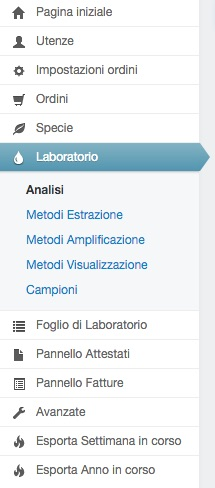
\includegraphics[width=0.3\textwidth]{images/suit}
  \end{center}
\end{wrapfigure}

Il pannello admin Django del Portale Avifauna deve permettere di controllare ogni passo del sistema.

\section*{Utenze}
Un utente del sistema é un entità identificata da un univoco indirizzo email, con password e nominativo. Esso ha attributi booleani per indicare se é attivo, se ha privilegi di staff o da superutente; é inoltre possibile indicare i singoli privilegi in un apposito elenco.

Un cliente invece é un entità associata ad un utente, con tutti gli attributi personali come nome, cognome, codice fiscale/partita iva, indirizzo, contatti telefonici e attributi di sistema come lo schema prezzi associato, la lingua oreferita, la quantità di crediti FEM in possesso e l'eventuale collegamento ad una associazione.

Le associazioni sono caratterizzate da un nome univoco, uno schema prezzi associato e eventuali informazioni aggiuntive.

Per indicare la correlazione tra cliente ed associazione esiste l'entità \texttt{iscrizione ad associazione} con il nominativo del cliente, l'associazione collegata e il numero di tessera corrispondente.

É stato inoltre aggiunto l'attributo booleano \texttt{ufficiale} per permettere agli addetti di {\fem} di indicare quando l'iscrizione del cliente all'associazione corrisponde al vero, poiché il registro degli iscritti di ogni associazione é aggiornato continuamente ma inviato a {\fem} solo ad intervalli temporali.

\section*{Impostazioni ordini}
In questa sezione si trovano quelle opzioni impostabili una tantum che non subiscono frequenti variazioni o controlli.

Vengono raccolti gli schemi di prezzi creati, indicati dal nome e contenenti le tariffe di ogni analisi e attestato; hanno la possibilità di essere di due tipi: Convenzioni o Pacchetti. 

Nel primo caso (tipico di associazioni o clienti professionisti che analizzano un range di specie ridotto) vengono impostati i costi delle analisi come convenzionati, l'ulteriore costo scontato in caso di superamento di una soglia minima dell'ordine e la soglia da superare; vengono anche elencate le specie sulle quali effettuare i prezzi favorevoli e quali invece mantengono il prezzo di listino.

Nel secondo caso invece vanno impostati anche i prezzi scontati di tutte le analisi da applicare in caso di combinazione tra più analisi richieste sullo stesso soggetto.

Vengono anche indicate le cifre dei pacchetti crediti FEM acquistabili, ovvero il prezzo di ciascuno e il credito che il cliente accumula.

Infine si possono impostare e modificare i \texttt{template messaggi}, cioè i messaggi pre-popolati che possono essere utilizzati nelle fasi di invio comunicazioni automatiche. Ogni template ha un nome identificativo univoco, descrizione e ordinamento opzionali e i corpi del testo divisi per ogni lingua.

\section*{Ordini}
Gli ordini sono descritti da campi non modificabili manualmente come lo stato, l'ammontare e il cliente associato; contengono note fiscali o interne, e mostrano la lista di campioni associati con la possibilità di indicare eventuali problematiche di ogni singolo campione. Viene fornita la possibilità di assegnare un \texttt{idLab} (numero sequenziale per il laboratorio) ad ogni campione

%\section*{Specie}

%\section*{Laboratorio}

%\section*{Foglio di laboratorio}

%\section*{Pannello attestati e Pannello fatture}

%\section*{Avanzate ed Esporta}